\documentclass[11pt]{scrartcl}
\usepackage{graphicx}
\pdfoutput=1
\usepackage{matlab-prettifier}
\usepackage{listings}
\usepackage{float}
\usepackage{tikz}
\usepackage[numbers,round]{natbib}
\usepackage{amsmath}
\usepackage{fancyhdr}
\usepackage{afterpage}
\usepackage{hyperref}
\usepackage{listings}
\usepackage{amsmath}

\usepackage{color}

\setcounter{secnumdepth}{4}
\setcounter{tocdepth}{4}   % Tiefe der Gliederung im In haltsverzeichnis
\pagestyle{fancy}
\renewcommand{\headrulewidth}{0.4pt}
\renewcommand{\footrulewidth}{0.4pt}
\fancyhf{} % clear all fields
\fancyhead[R]{}
\fancyfoot[C]{\thepage}
\fancypagestyle{plain}{%
	\renewcommand{\headrulewidth}{0.4pt}%
	\renewcommand{\footrulewidth}{0.4pt}%
	\fancyhf{}% clear all fields
	\fancyhead[R]{Emrah Öztürk}%
	\fancyfoot[C]{\thepage}%
}


\definecolor{mygreen}{rgb}{0,0.6,0}
\definecolor{mygray}{rgb}{0.5,0.5,0.5}
\definecolor{mymauve}{rgb}{0.58,0,0.82}

\definecolor{mygreen}{RGB}{28,172,0} % color values Red, Green, Blue
\definecolor{mylilas}{RGB}{170,55,241}

\lstset{language=Matlab,%
	%basicstyle=\color{red},
	breaklines=true,%
	morekeywords={matlab2tikz},
	keywordstyle=\color{blue},%
	morekeywords=[2]{1}, keywordstyle=[2]{\color{black}},
	identifierstyle=\color{black},%
	stringstyle=\color{mylilas},
	commentstyle=\color{mygreen},%
	showstringspaces=false,%without this there will be a symbol in the places where there is a space
	numbers=left,%
	numberstyle={\tiny \color{black}},% size of the numbers
	numbersep=9pt, % this defines how far the numbers are from the text
	emph=[1]{for,end,break},emphstyle=[1]\color{red}, %some words to emphasise
	emph=[2]{word1,word2}, emphstyle=[2]{style},    
}

\begin{document}
	\section*{calculations relative green}
	
	We have the following green phases in each intersection. 
	
	\begin{figure}[H]
		\centering
		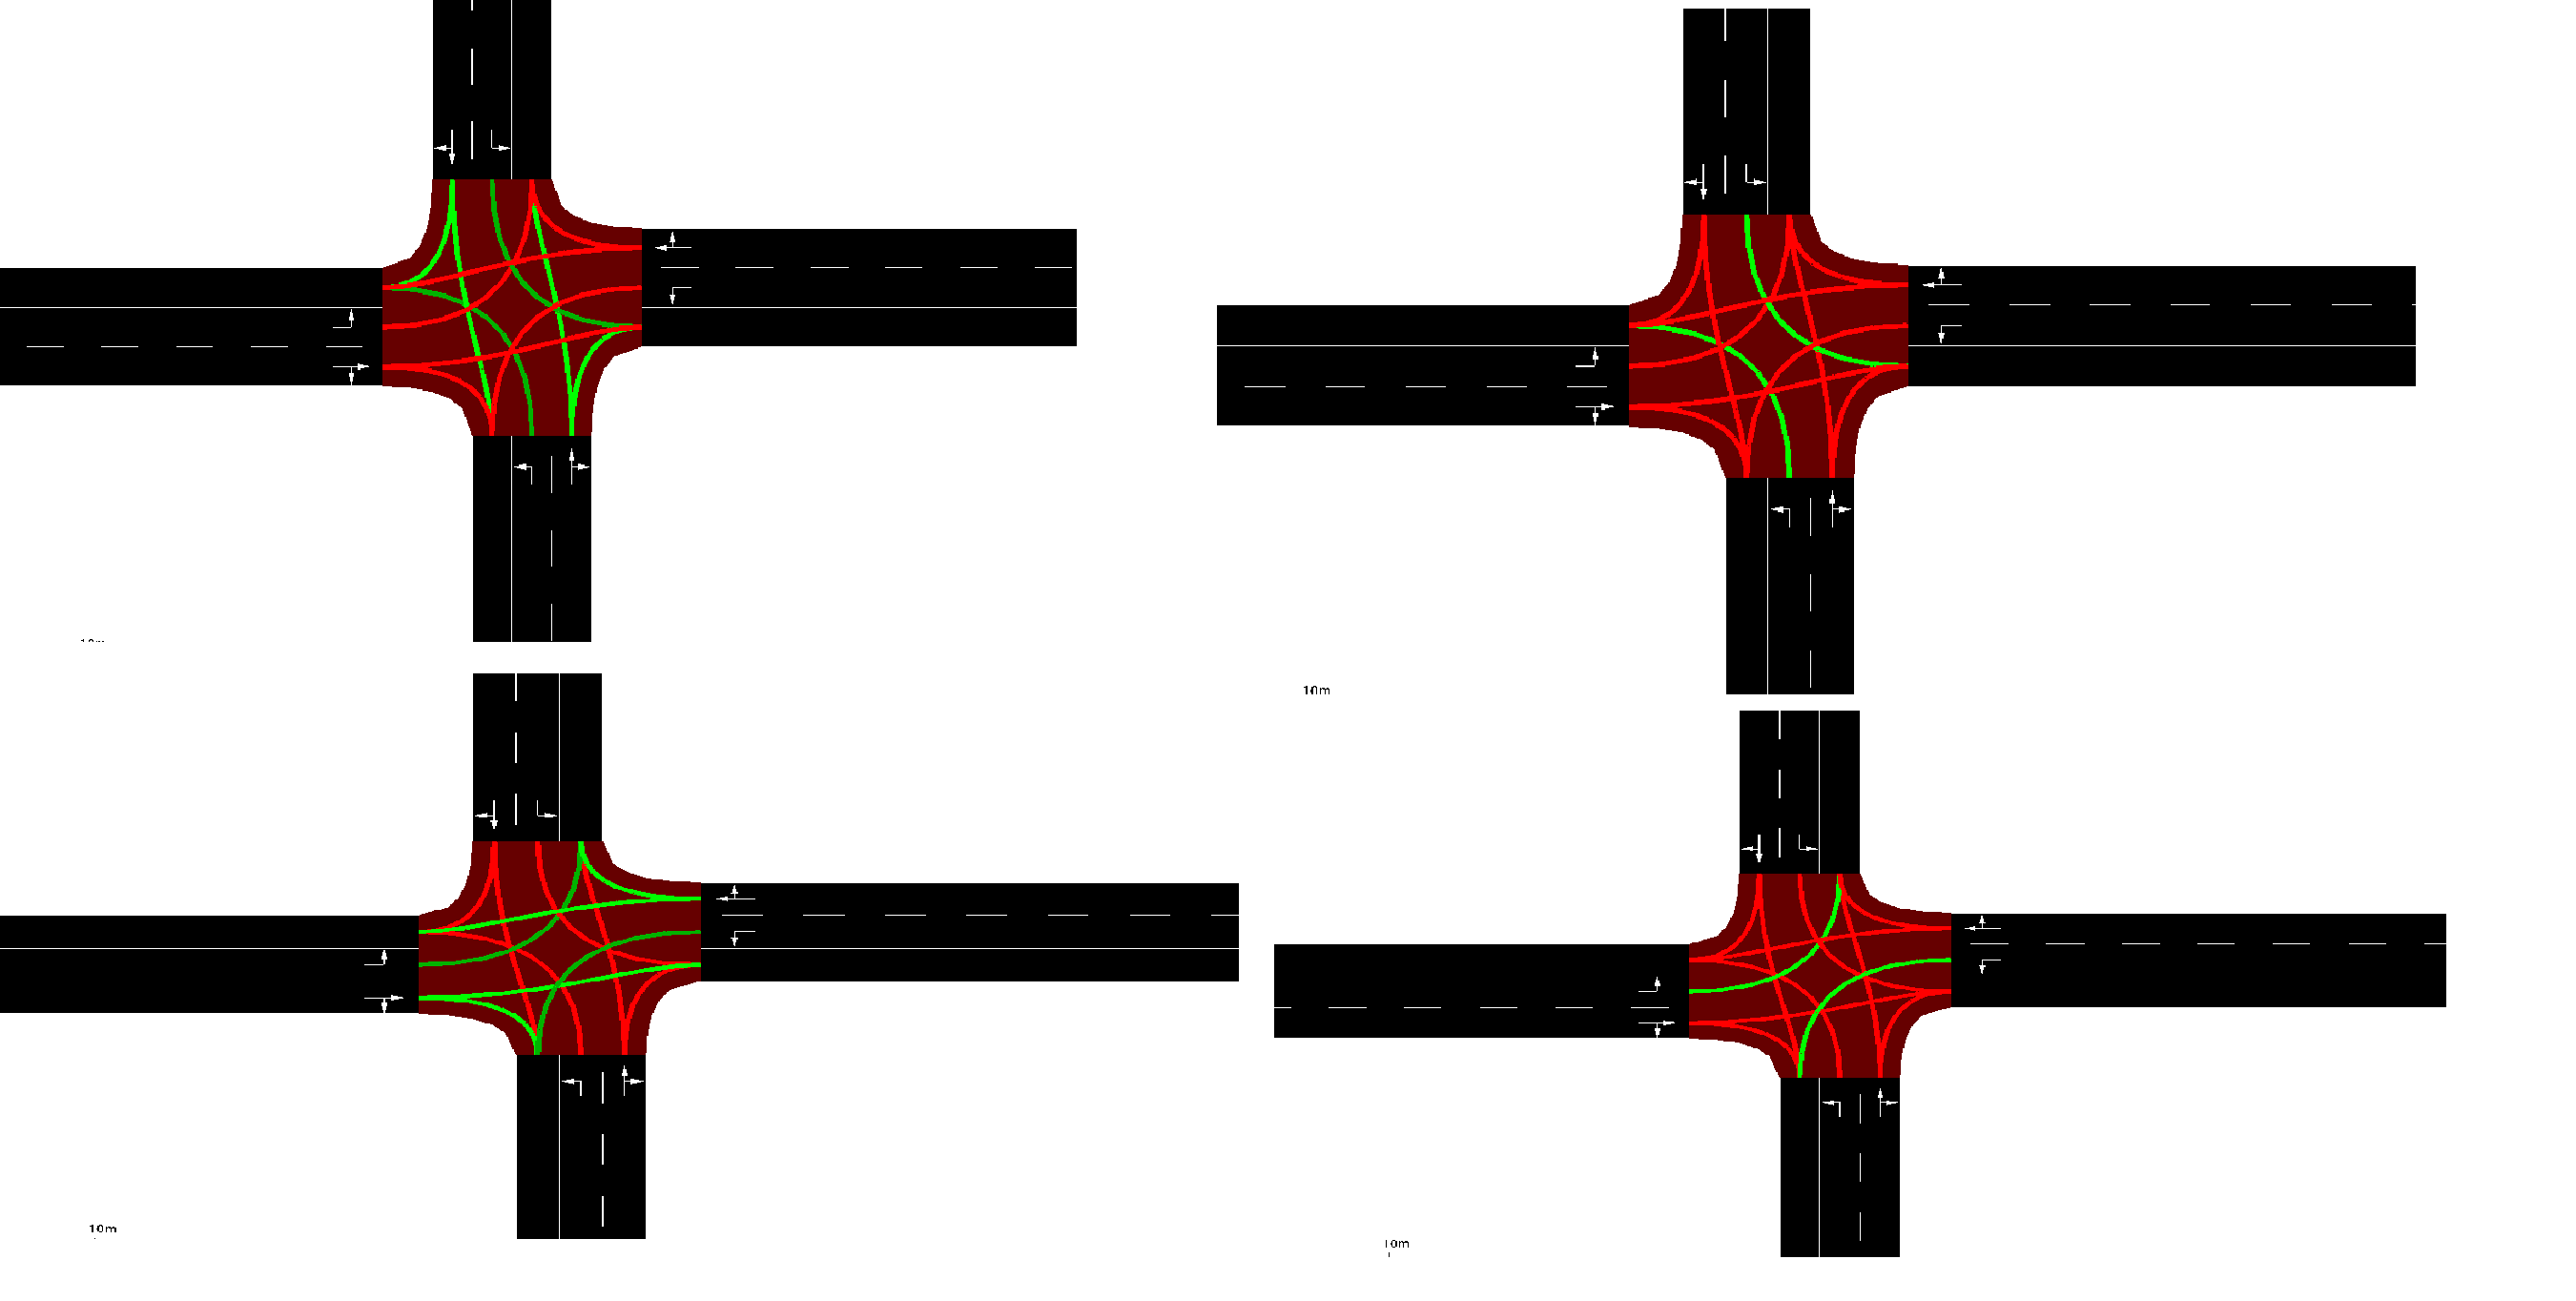
\includegraphics[width=1.2\linewidth]{greenPhases}
		\caption{different green phases in 3x3 intersection}
		\label{fig:greenphases}
	\end{figure}
	
	The calculation of the relative greens is related to the input stream in an intersection. If we call the input stream from the street i $I_{i}$ and the turn probability from the i-th street to the j-th street $p_{ij}$ then we can determine the relative green time using an weighted average. Note that the streets are numerated from 1 (north) increasing clockwise to 4 (west). For the first relative green time (figure 1 upper left) we get the following calculation
	
	\begin{equation}\label{key}
	rg_{phase 1} = \frac{max(I_{1}(p_{13} + p_{14})+I_{3}(p_{31}+p_{32}))}{\sum_{i=1}^{4}phase_{i}} 
	\end{equation}
	
	This is because, we have an input stream from street 1 divided (according to the turn probability's) into street 3 ($I_{1}p_{13}$) and street 4 ($I_{1}p_{14}$). The same is done for the input stream $I_{3}$. Then this value is divided by the sum of all green phases. This procedure is then used to calculate all four phases.
	
	
\end{document}